\documentclass{standalone}
\usepackage{tikz}
\usetikzlibrary{arrows}

\begin{document}
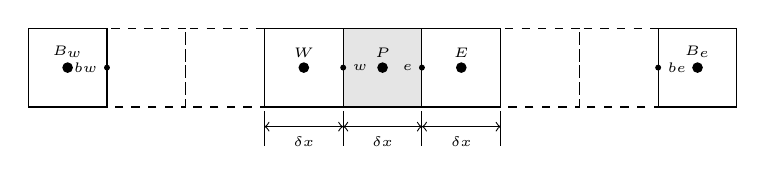
\begin{tikzpicture}
    \draw (0,0) rectangle (1,1);
    \draw[dashed] (1,0) rectangle (2,1);
    \draw[dashed] (2,0) rectangle (3,1);
    \draw (3,0) rectangle (4,1);
    \filldraw[fill=gray!20,draw=black] (4,0) rectangle (5,1);
    \draw (5,0) rectangle (6,1);
    \draw[dashed] (6,0) rectangle (7,1);
    \draw[dashed] (7,0) rectangle (8,1);
    \draw (8,0) rectangle (9,1);
    
    \filldraw (0.5,0.5) circle (0.06) node[above] {\tiny{}$B_w$};
    \filldraw (3.5,0.5) circle (0.06) node[above] {\tiny{}$W$};
    \filldraw (4.5,0.5) circle (0.06) node[above] {\tiny{}$P$};
    \filldraw (5.5,0.5) circle (0.06) node[above] {\tiny{}$E$};
    \filldraw (8.5,0.5) circle (0.06) node[above] {\tiny{}$B_e$};
    
    \filldraw (1,0.5) circle (0.03) node[left] {\tiny{}$bw$};
    \filldraw (4,0.5) circle (0.03) node[right] {\tiny{}$w$};
    \filldraw (5,0.5) circle (0.03) node[left] {\tiny{}$e$};
    \filldraw (8,0.5) circle (0.03) node[right] {\tiny{}$be$};
    
    \draw (3,-0.05) -- (3,-0.5);
    \draw (4,-0.05) -- (4,-0.5);
    \draw (5,-0.05) -- (5,-0.5);
    \draw (6,-0.05) -- (6,-0.5);
    
    \draw[<->] (3,-0.25) -- (4,-0.25) node[below] at (3.5,-0.25){\tiny{}$\delta{}x$};
    \draw[<->] (4,-0.25) -- (5,-0.25) node[below] at (4.5,-0.25){\tiny{}$\delta{}x$};
    \draw[<->] (5,-0.25) -- (6,-0.25) node[below] at (5.5,-0.25){\tiny{}$\delta{}x$};
\end{tikzpicture}
\end{document}